
\chapter{Requirements specification}

\label{ch:requirements}
\lhead{Chapter 4. \emph{Requirements specification}}

This chapter provides a description of project's stakeholders and requirements, both
functional and non-functional. Requirements will be presented textually and with the aid of
some use-case diagrams.

Throughout this chapter both requirement's priority and complexity have a textual description which can be
\begin{itemize}
\item High
\item Medium (abbrev. Med)
\item Low
\end{itemize}

The use of such terms is described in table \ref{table:priorities} for priorities
and table \ref{table:complexity} for complexities.
\begin{table}[H]
\begin{center}
\begin{tabular}{ | r | p{11.5cm} | }
  \hline
  \textbf{Priority} & \textbf{Description} \\
  \hline\noalign{\smallskip}\noalign{\smallskip}\hline
  \textbf{High} & An essential requirement.\newline
  The product \textbf{must fulfill} the requirement in order to be satisfactory. \\
  \textbf{Medium} & A useful requirement.\newline
  The product \textbf{should fulfill} the requirement to maximise effectiveness. \\
  \textbf{Low} & A desiderable requirement.\newline
  The product \textbf{could fulfill} the requirement to be more interesting to some stakeholders. \\
  \hline
\end{tabular}
\end{center}
\caption{Priority descriptions}
\label{table:priorities}
\end{table}

\begin{table}[H]
\begin{center}
\begin{tabular}{ | r | p{11.5cm} | }
  \hline
  \textbf{Complexity} & \textbf{Description} \\
  \hline\noalign{\smallskip}\noalign{\smallskip}\hline
  \textbf{High} & The requirement is difficult to implement.\newline
  It will take a considerable amount of time. (more than 45 hours) \\
  \textbf{Medium} & The requirement is moderately difficult.\newline
  It will take some time. (from 15 to 45 hours) \\
  \textbf{Low} & The requirement is easy and can be achieved\newline
  in a short amount of time. (15 hours or less) \\
  \hline
\end{tabular}
\end{center}
\caption{Complexity descriptions}
\label{table:complexity}
\end{table}


%-----

\section{Stakeholders}
\label{section:stakeholders}
A project's stakeholders are those people that have an interest in the project.
%This section contains a description of project's stakeholders: those people that have an interest in it.
We have identified five stakeholders for this project and presented them below.
%A short description\iffalse of the role\fi of each stakeholder is given, and what concerns they might have.

\subsection{Customer}
The customer is\iffalse the one that is\fi going to steer the project toward the direction he pleases.
The interest of the customer is to receive a product that will be as useful as possible for him.
% us to the solution he wants.
%His concern is that we should maintain an effective and good communication with him, so he understands our progress.
His concern is to be able to communicate well with the group and make his expectations for the product
and for the documentation clear.
%We should also document the advancement we are making and have a clear system architecture for him.
%His main concern is to get a working prototype of our system according to his requirements.

\subsection{Course's staff}
The course's staff will evaluate our project. Their interest is that we, as a group of students,
gain valuable knowledge and experience in a number of areas related to software development.
It is their interest to make the criterias behind grading clear to the students
so that their effort is focused on the objectives of the course.
They expect all the deliverables to be submitted on schedule.
%Good communication is also of importance, and of course that we will learn something from the course.

\subsection{Our group}
As a group made up of good students, our main interest is to gain the most out of our tuition.
We have therefore committed to pass this course with a good profit and will give our best
to satisfy the customer and produce a good documentation.
%We are going to write the report and implement our applications.
%Our concern is to fulfil the requirements of our customer, finish the report and have a good presentation
%that reflects our work.

\subsection{Third party developers}
The third party developers are going to integrate their applications with our system, or eventually
extend some of its functionality. Their concern is that our integration platform is well documented
in order to be easy to integrate with or to extend.

\subsection{Users}
The users are going to user product: the front-end and Android applications.
%They are the users of our front-end and both Android applications.%heart rate application and our weight application.
It is their concern that their data is easily available and is visualized in an intuitive and comprehensible way.
They should be able to push heart rate and weight measurements to the integration platform smoothly and without
any explicit training.

%-----

\newpage
\section{Funcional requirements}
\label{section:functionalreq}

This section contains a description the functional requirements for the product.
Each requirement also had a priority which helped us identify the focus of our work.
Priorities can be reviewed based on customer's feedback. We tried to prioritize those requirements corresponding
to the functionality of the system that the customer expressed most interest about. In order to better organize
our workload we also assigned a \'difficulty\' to each requirement.

\textbf{Functional requirements for Integration Platform}

\begin{table}[H]
\begin{center}
\begin{tabular}{ | r | p{11.5cm} | }
  \hline

  \textbf{ID} & FIP1 \\
  \hline\noalign{\smallskip}\hline
  \textbf{Description}  & The IP shall support API endpoints for receiving heart rate data
                          models expressed as JSON strings.\\
  \textbf{Complexity}   & Med \\
  \textbf{Priority}     & High \\
  \hline\noalign{\smallskip}\noalign{\smallskip}\hline

  \textbf{ID} & FIP2 \\
  \hline\noalign{\smallskip}\hline
  \textbf{Description}  & The IP shall support API endpoints for receiving
                          weight data models expressed as JSON strings.\\
  \textbf{Complexity}   & Med \\
  \textbf{Priority}     & High \\
  \hline\noalign{\smallskip}\noalign{\smallskip}\hline

  \textbf{ID} & FIP3 \\
  \hline\noalign{\smallskip}\hline
  \textbf{Description}  & The IP shall support API endpoints for forwarding
                          stored heart rate measurements as JSON models.\\
  \textbf{Complexity}   & Med \\
  \textbf{Priority}     & High \\
  \hline\noalign{\smallskip}\noalign{\smallskip}\hline

  \textbf{ID} & FIP4 \\
  \hline\noalign{\smallskip}\hline
  \textbf{Description}  & The IP shall support API endpoints for forwarding
                          stored weight measurements as JSON models.\\
  \textbf{Complexity}   & Med \\
  \textbf{Priority}     & High \\

  \iffalse
  ID & Description & Difficulty & Priority\\
  \hline\noalign{\smallskip}\noalign{\smallskip}\hline
  FIP1	& The IP shall support API endpoints for receiving
          heart rate data models expressed as JSON strings.		& Med	& High \\
  FIP2	& The IP shall support API endpoints for receiving
          weight data models expressed as JSON strings.				& Med	& High \\
  FIP3	& The IP shall support API endpoints for forwarding
          stored heart rate measurements as JSON models.			& Med	& High \\
  FPI4	& The IP shall support API endpoints for forwarding
          stored weight measurements as JSON models.					& Med	& High \\
  \fi

  \hline
\end{tabular}
\end{center}
\caption{Functional requirements for Integration Platform}
\label{table:reqip}
\end{table}


\textbf{Functional requirements for the web frontend}

\begin{table}[H]
\begin{center}
\begin{tabular}{ | r | p{11.5cm} | }
  \hline

  \textbf{ID} & FW1 \\
  \hline\noalign{\smallskip}\hline
  \textbf{Description}  & The web frontend shall display the data stored by the Integration Platform using charts.\\
  \textbf{Complexity}   & Med \\
  \textbf{Priority}     & High \\
  \hline\noalign{\smallskip}\noalign{\smallskip}\hline

  \textbf{ID} & FW2 \\
  \hline\noalign{\smallskip}\hline
  \textbf{Description}  & The web frontend shall use Helsenorge color palette. \\
  \textbf{Complexity}   & Low \\
  \textbf{Priority}     & Low \\
  
  \hline
\end{tabular}
\end{center}
\caption{Functional requirements for the web frontend}
\label{table:reqfrontend}
\end{table}

\newpage
\textbf{Functional requirements for Heart rate application}

\begin{table}[H]
\begin{center}
\begin{tabular}{ | r | p{11.5cm} | }
  \hline

  \textbf{ID} & FHR1 \\
  \hline\noalign{\smallskip}\hline
  \textbf{Description}  & The application shall measure user's heart rate using the device camera.\\
  \textbf{Complexity}   & High \\
  \textbf{Priority}     & High \\
  \hline\noalign{\smallskip}\noalign{\smallskip}\hline

  \textbf{ID} & FHR2 \\
  \hline\noalign{\smallskip}\hline
  \textbf{Description}  & The application shall display the measurement on screen. \\
  \textbf{Complexity}   & Low \\
  \textbf{Priority}     & High \\
  \hline\noalign{\smallskip}\noalign{\smallskip}\hline

  \textbf{ID} & FHR3 \\
  \hline\noalign{\smallskip}\hline
  \textbf{Description}  & The application shall forward the data to the IP using its REST endpoint.\\
  \textbf{Complexity}   & Med \\
  \textbf{Priority}     & High \\
  
  \hline
\end{tabular}
\end{center}
\caption{Functional requirements for heart rate application}
\label{table:reqheartrate}
\end{table}


\newpage
\textbf{Functional requirements for Weight application}

\begin{table}[H]
\begin{center}
\begin{tabular}{ | r | p{11.5cm} | }
  \hline
  
  \textbf{ID} & FHV1 \\
  \hline\noalign{\smallskip}\hline
  \textbf{Description}  & The application shall fetch weight data from HealthVault. \\
  \textbf{Complexity}   & Med \\
  \textbf{Priority}     & High \\
  \hline\noalign{\smallskip}\noalign{\smallskip}\hline

  \textbf{ID} & FHV2 \\
  \hline\noalign{\smallskip}\hline
  \textbf{Description}  & The application shall display the data it has fetched. \\
  \textbf{Complexity}   & Low \\
  \textbf{Priority}     & Med \\
  \hline\noalign{\smallskip}\noalign{\smallskip}\hline

  \textbf{ID} & FHV3 \\
  \hline\noalign{\smallskip}\hline
  \textbf{Description}  & The application shall forward the data to the IP using the web API. \\
  \textbf{Complexity}   & Low \\
  \textbf{Priority}     & High \\

  \iffalse
  ID & Description & Difficulty & Priority\\
  \hline\noalign{\smallskip}\noalign{\smallskip}\hline
  FHV1	& The application shall fetch weight data from HealthVault.						      & Med	& High \\
  FHV2	& The application shall show the user the data it has fetched.              & Low	& Med \\
  FHV3	& The application shall forward the data to the IP using its REST endpoint. & Med	& High \\
  \fi

  \hline
\end{tabular}
\end{center}
\caption{Functional requirements for the weight application}
\label{table:reqweight}
\end{table}

\textbf{Functional requirements for HealthVault Integration Service}

\begin{table}[H]
\begin{center}
\begin{tabular}{ | r | p{11.5cm} | }
  \hline
  
  \textbf{ID} & FHIS1 \\
  \hline\noalign{\smallskip}\hline
  \textbf{Description}  &  The user shall be able to turn the application on and off. \\
  \textbf{Complexity}   & Low \\
  \textbf{Priority}     & Med \\
  \hline\noalign{\smallskip}\noalign{\smallskip}\hline

  \textbf{ID} & FHIS2 \\
  \hline\noalign{\smallskip}\hline
  \textbf{Description}  & When on, the applicatin shall fetch weight data from HealthVault and
                          forward it to the IP using its web API. \\
  \textbf{Complexity}   & Med \\
  \textbf{Priority}     & High \\
  \hline\noalign{\smallskip}\noalign{\smallskip}\hline

  \textbf{ID} & FHIS3 \\
  \hline\noalign{\smallskip}\hline
  \textbf{Description}  & The application shall allow the user to manually send weight measurements to HealthVault. \\
  \textbf{Complexity}   & Low \\
  \textbf{Priority}     & Med \\

\iffalse
\begin{table}[H]
\begin{center}
\begin{tabular}{ | c | p{9cm} | c | c |}
  \hline
  ID & Description & Difficulty & Priority\\
  \hline\noalign{\smallskip}\noalign{\smallskip}\hline
  FHIS1	& The application shall send weight data to HealthVault.						   & Low	& Low \\
  FHIS2	& The application shall fetch weight data from HealthVault regularly.		       & Med	& High \\
  FHIS3	& The application shall forward new weight data to the IP using its REST endpoint. & Med	& High \\
  \hline
\end{tabular}
\end{center}
\caption{Functional requirements for HealthVault Integration Service}
\label{table:reqwebservice}
\end{table}
\fi

  \hline
\end{tabular}
\end{center}
\caption{Functional requirements for the weight application}
\label{table:reqwebservice}
\end{table}

%-----
\newpage
\section{Non-functional requirements}
\label{section:nonfunctionalreq}

This section outlines non-functional requirements (quality attributes) for the product.
In order to provide a better overview, we have organized them in categories.


\begin{table}[H]
\begin{center}
\begin{tabular}{ | r | p{11.5cm} | }
  \hline
  
  \textbf{ID} & NF1 \\
  \hline\noalign{\smallskip}\hline
  \textbf{Category}			&	Documentation\\
  \textbf{Description}	& The system shall be thoroughly documented by the 'project report' \\
  \textbf{Complexity}		& High \\
  \textbf{Priority}			& High \\
  \hline\noalign{\smallskip}\noalign{\smallskip}\hline

  \textbf{ID} & NF2 \\
  \hline\noalign{\smallskip}\hline
  \textbf{Category}			&	Documentation\\
  \textbf{Description}	& Although security and privacy are not requirements for the product they
													are important topics to be discussed in the documentation. \\
  \textbf{Complexity}		& Med \\
  \textbf{Priority}			& High \\
  \hline\noalign{\smallskip}\noalign{\smallskip}\hline

  \textbf{ID} & NF3 \\
  \hline\noalign{\smallskip}\hline
  \textbf{Category}			&	Open-source\\
  \textbf{Description}	& The product shall be released under a permissive license approved by the product owner. \\
  \textbf{Complexity}		& Med \\
  \textbf{Priority}			& Med \\
  \hline\noalign{\smallskip}\noalign{\smallskip}\hline
  
  \textbf{ID} & NF4 \\
  \hline\noalign{\smallskip}\hline
  \textbf{Category}			&	Interoperability \\
  \textbf{Description}	& The system shall provide a good degree of interoperability.
  												Third party application developers should be put in the condition to develop
  												third party (interoperable) solutions rapidly. \\
  \textbf{Complexity}		& High \\
  \textbf{Priority}			& High \\

  \hline
\end{tabular}
\end{center}
\caption{Non-functional requirements}
\label{table:nonfunc}
\end{table}

\begin{table}[H]
\begin{center}
\begin{tabular}{ | r | p{11.5cm} | }
	\hline

  \textbf{ID} & NF5 \\
  \hline\noalign{\smallskip}\hline
  \textbf{Category}     & Interoperability \\
  \textbf{Description}  & A number of two or three prototype applications shall be developed in order to showcase
                          the functionality of the system \\
  \textbf{Complexity}   & High \\
  \textbf{Priority}     & High \\
  \hline\noalign{\smallskip}\noalign{\smallskip}\hline
	
	\textbf{ID} & NF6 \\
  \hline\noalign{\smallskip}\hline
  \textbf{Category}			&	Accessibility \\
  \textbf{Description}	& The web-frontend should have a good degree of accessibility.
  												It should have a rather simple design and use a customer-provided palette. \\
  \textbf{Complexity}		& Low \\
  \textbf{Priority}			& Low \\
	
	\hline
\end{tabular}
\end{center}
\caption{Non-functional requirements (cont.)}
\end{table}

%% old format table, commented out
\iffalse
\begin{table}[H]
\begin{center}
\begin{tabular}{ | c | c |p{6.5cm} | c | c |}
  \hline
  ID & Category & Description & Difficulty & Priority\\
  \hline\noalign{\smallskip}\noalign{\smallskip}\hline
  NF1 & Documentation & The system shall be thoroughly documented by the document 'project report'.
  & High & High \\
  \hline
  NF2 & Documentation & Although security and privacy are not requirements for the product they
  are important topics to be discussed in the documentation.
  & Med & High \\
  \hline
  NF3 & Open-source	& The product shall be released under a permissive license approved by the product owner.
  & Low & High \\
  \hline
  NF4 & Interoperability & The system shall provide a good degree of interoperability.
  Third party application developers should be put in the condition to develop third party (interoperable)
  solutions rapidly.
  & High & High \\
  \hline
  NF5 & Interoperability & A number of two or three prototype applications shall be developed in order to showcase
  the functionality of the system.
  & High & High \\
  \hline
  NF6 & Accessibility & The web-frontend should have a good degree of accessibility. It should have a rather simple
  design and use a customer-provided palette.
  & Low & Low \\
  \hline
\end{tabular}
\end{center}
\caption{Non-functional requirements}
\label{table:reqnonfunc}
\end{table}
\fi

% -----

\section{Requirements Validation}
\label{section:reqvalidation}

This section contains some considerations we made when defining requirements to ensure their validity\cite{Sommerville9}.

\textbf{Comprehensibility}\newline
It is important that requirements are expressed in a way that is understandable by the customer.
We have thus submitted a list of both functional and non-functional requirements of the system
to the customer for approval. Because requirements were subject to change due to the nature of the project
itself, the customer has reviewed them multiple times.

\textbf{Verifiability}\newline
It is crucial that a requirement can be tested. If a requirement can't be tested, it is not a valid requirement.
We have kept this in mind while formalising requirements.

\textbf{Adaptability (changeability)}\newline
We expected requirements to change multiple times during development.
For this reason we started with a set of high-level requirements to be later refined and improved.
This would allow the requirements to change without having a big impact on the progress of the project.

%-----

\section{Use cases}
\label{section:usecases}

This section provides  the different use cases of our applications.
The section consists of use cases for the front-end, heart rate application and the weight application.

\subsection{Front-end}

The use case diagram for the front-end is shown in figure \ref{figure:use-case-diagram-front-end}.
From the use case diagram we see that the front-end has two main objectives.
The first one is to fetch data from our integration platform, and the second one is to display this data to the user.
In table \ref{table:use-case-view-data} we present a textual use case for the front-end.

\begin{figure}[H]
\centering
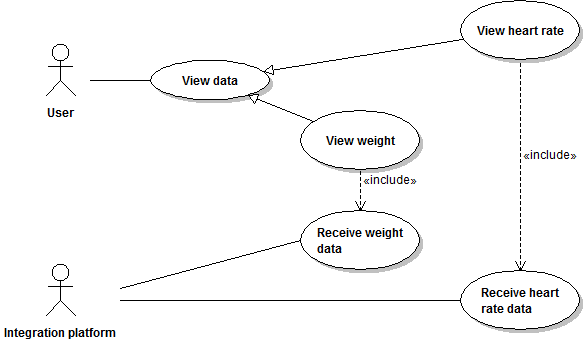
\includegraphics[scale=0.6]{../Figures/use-case-diagram-front-end.png}
\caption{Use case diagram - Front-end}
\label{figure:use-case-diagram-front-end}
\end{figure}

\begin{table}[H]
\begin{center}
\begin{tabular}{ l | p{10cm} }
  \hline
  \textbf{Use Case Element} & \textbf{Description} \\ \hline\hline
  Requirements & \hyperref[table:reqfrontend]{FW1}, \hyperref[table:reqip]{FIP3} and \hyperref[table:reqip]{FIP4}\\ \hline
  Application & Front-end \\ \hline
  Name & View data \\ \hline
  Description & Display all the data from the integration platform for the user. \\ \hline
  Actor & User and Integration Platform \\ \hline
  Precondition &
	\par 1. The integration platform has data about the current user.
	\par 2. The integration platform is online.
	\par 3. The user is using a computer with a web browser, that is connected to the internet.
	\\ \hline
  Basic Flow & 
  	\par 1. The user accesses the web page.
  	\par 2. Front-end requests data from the integration platform.
  	\par 3. Integration platform sends data to front-end.
  	\par 4. Front-end displays data to user.
  	\\ \hline
  Alternate Flows & 
  	\par 1A: The user wants to only view heart rate data.
  	\par\hspace{15pt} 1. The user clicks on \textit{Heart Rate} in the navigation bar.
  	\par 1B: The user wants to only view weight data.
  	\par\hspace{15pt} 1. The user clicks on \textit{Weight} in the navigation bar.
  \\ \hline
\end{tabular}
\end{center}
\caption{Textual use case - View data}
\label{table:use-case-view-data}
\end{table}

\subsection{Heart Rate Application}

A use case diagram for the heart rate application is given in figure \ref{figure:use-case-diagram-heart-rate}.
The main objectives of this application is to measure and send the data to the integration platform.

\begin{figure}[H]
\centering
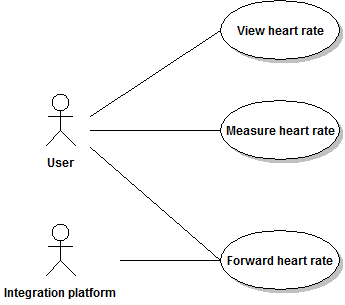
\includegraphics[scale=0.6]{../Figures/use-case-diagram-heart-rate.png}
\caption{Use case diagram - Heart rate application}
\label{figure:use-case-diagram-heart-rate}
\end{figure}

A textual use case for measuring and viewing the heart rate is given in table \ref{table:use-case-measure-heart-rate}.
Figure \ref{figure:use-case-diagram-measure-heart-rate} shows a use case diagram for the textual use case.

\begin{figure}[H]
\centering
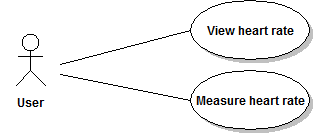
\includegraphics[scale=0.75]{../Figures/use-case-diagram-measure-and-view-heart-rate.png}
\caption{Use case diagram - Measure and view heart rate}
\label{figure:use-case-diagram-measure-heart-rate}
\end{figure}

\begin{table}[H]
\begin{center}
\begin{tabular}{ l | p{10cm} }
  \hline
  \textbf{Use Case Element} & \textbf{Description} \\ \hline\hline
  Requirements & \hyperref[table:reqheartrate]{FHR1} and \hyperref[table:reqheartrate]{FHR2} \\ \hline
  Application & Heart Rate Application \\ \hline
  Name & Measure and view heart rate \\ \hline
  Description & Measure the heart rate of the user and then view the measured data. \\ \hline
  Actor & User \\ \hline
  Precondition &
    \par 1. The users phone meets the requirements of the heart rate application.
  	\par 2. The application is installed on the users phone.
  	\par 3. The application is running on the users phone.
  \\ \hline
  Basic Flow & 
  	\par 1. The user places his finger on the camera of the phone.
  	\par 2. The user waits until the heart rate is shown on the display.
  	\par 3. The user views the heart rate.
  \\ \hline
  Alternate Flows & 
  	\par 1A: The user places his finger wrongly, which makes the measured data incorrect.
  	\par\hspace{15pt} 1. The user adjusts his finger.
  \\ \hline
\end{tabular}
\end{center}
\caption{Textual use case - Measure and view heart rate}
\label{table:use-case-measure-heart-rate}
\end{table}

Table \ref{table:use-case-send-heart-rate} gives a textual use case for sending the heart rate to the integration platform.
Figure \ref{figure:use-case-diagram-send-heart-rate} shows a use case diagram for the textual use case.

\begin{figure}[H]
\centering
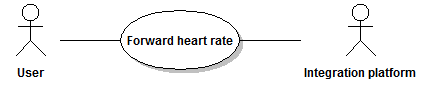
\includegraphics[scale=0.75]{../Figures/use-case-diagram-send-heart-rate.png}
\caption{Use case diagram - Send heart rate}
\label{figure:use-case-diagram-send-heart-rate}
\end{figure}

\begin{table}[H]
\begin{center}
\begin{tabular}{ l | p{10cm} }
  \hline
  \textbf{Use Case Element} & \textbf{Description} \\ \hline\hline
  Requirements & \hyperref[table:reqheartrate]{FHR3} and \hyperref[table:reqip]{FIP1} \\ \hline
  Application & Heart Rate Application \\ \hline
  Name & Send heart rate \\ \hline
  Description & Send the measured heart rate to the integration platform. \\ \hline
  Actor & User and Integration Platform \\ \hline
  Precondition &
    \par 1. The user has measured his/hers heart rate through the application.
    \par 2. The phone is connected to the internet.
    \par 3. The integration platform is online.
  \\ \hline
  Basic Flow & 
  	\par 1. The user clicks on \textit{Send}.
  	\par 2. The application sends the data to the integration platform.
  	\par 3. The integration platform receives the data.
  \\ \hline
\end{tabular}
\end{center}
\caption{Textual use case - Send heart rate}
\label{table:use-case-send-heart-rate}
\end{table}

\subsection{Weight Application}

The goal of the weight application is to retrieve weight data from HaulthVault and forward it to our integration platform.
Figure \ref{figure:use-case-diagram-weight} shows the main use case diagram for the application.

\begin{figure}[H]
\centering
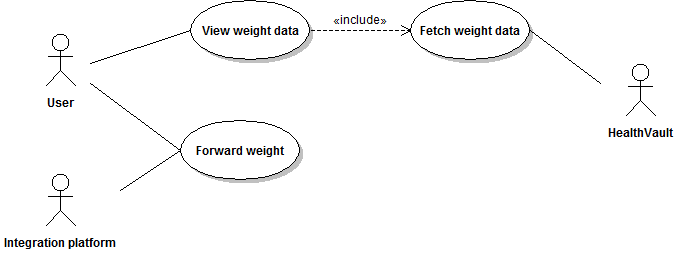
\includegraphics[scale=0.6]{../Figures/use-case-diagram-weight.png}
\caption{Use case diagram - Weight application}
\label{figure:use-case-diagram-weight}
\end{figure}

In figure \ref{figure:use-case-diagram-view-weight} a use case diagram is given for fetching and viewing the weight data.
Table \ref{table:use-case-view-weight-data} gives a textual use case for the use case diagram.

\begin{figure}[H]
\centering
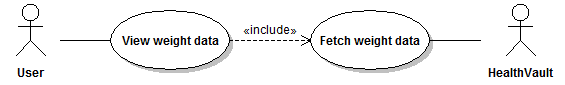
\includegraphics[scale=0.75]{../Figures/use-case-diagram-view-weight.png}
\caption{Use case diagram - View weight data}
\label{figure:use-case-diagram-view-weight}
\end{figure}

\begin{table}[H]
\begin{center}
\begin{tabular}{ l | p{10cm} }
  \hline
  \textbf{Use Case Element} & \textbf{Description} \\ \hline\hline
  Requirements & \hyperref[table:reqweight]{FHV1} and \hyperref[table:reqweight]{FHV2}\\ \hline
  Application & Weight Application \\ \hline
  Name & View weight data \\ \hline
  Description & Fetch the weight data from HealthVault and display it for the user. \\ \hline
  Actor & User and HealthVault \\ \hline
  Precondition &
    \par 1. The users phone meets the requirements of the weight application.
  	\par 2. The application is installed on the users phone.
  	\par 3. The application is running on the users phone.
  	\par 4. The application is connected to the internet.
  \\ \hline
  Basic Flow & 
  	\par 1. The user writes his email to HealthVault into the email field.
  	\par 2. The user writes his password to HealthVault into the password field.
  	\par 3. The user clicks on a button to login.
  	\par 4. The application shows the data for the user.
  	\par 5. The user views the data.
  \\ \hline
  Alternate Flows & 
  	\par 3A: The user inputs an invalid password or email.
  	\par\hspace{15pt} 1. The user has to go back to step 1 and start over again.
  \\ \hline
\end{tabular}
\end{center}
\caption{Textual use case - View weight data}
\label{table:use-case-view-weight-data}
\end{table}

Table \ref{table:use-case-send-weight-data} gives a textual use case for sending the weight data to our
integration platform. Figure \ref{figure:use-case-diagram-send-weight} displays a use case diagram for the
textual use case.

\begin{figure}[H]
\centering
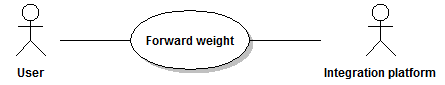
\includegraphics[scale=0.75]{../Figures/use-case-diagram-send-weight.png}
\caption{Use case diagram - Send weight data}
\label{figure:use-case-diagram-send-weight}
\end{figure}

\begin{table}[H]
\begin{center}
\begin{tabular}{ l | p{10cm} }
  \hline
  \textbf{Use Case Element} & \textbf{Description} \\ \hline\hline
  Requirements & \hyperref[table:reqweight]{FHV3} and \hyperref[table:reqip]{FIP2}\\ \hline
  Application & Weight Application \\ \hline
  Name & Send weight data \\ \hline
  Description & Send the weight data from the phone application into the integration platform. \\ \hline
  Actor & User and Integration Platform \\ \hline
  Precondition &
    \par 1. The user has acquired the weight data through the weight application.
    \par 2. The integration platform is online.
  \\ \hline
  Basic Flow & 
  	\par 1. The user presses the \textit{Send} button.
  	\par 2. The integration platform receives the data.
  \\ \hline
\end{tabular}
\end{center}
\caption{Textual use case - Send weight data}
\label{table:use-case-send-weight-data}
\end{table}

\subsection{HealthVault Integration Service}

The goal of the HealthVault Integration Service is to poll data regularly from HealthVault.
If a new value is detected then it is sent to the integration platform.
The web service should also be capable of sending weight values to HealthVault.
Figure \ref{figure:use-case-diagram-weight-service} shows a use case diagram of the system.

\begin{figure}[H]
\centering
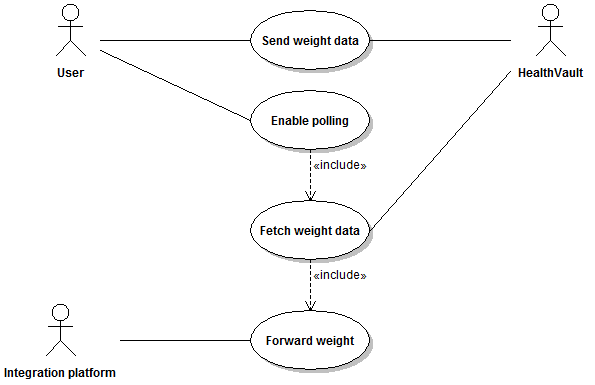
\includegraphics[scale=0.75]{../Figures/use-case-diagram-weight-service.png}
\caption{Use case diagram - HealthVault Integration Service}
\label{figure:use-case-diagram-weight-service}
\end{figure}

Figure \ref{figure:use-case-diagram-weight-service-send} shows a use case diagram for the sending functionality, while table \ref{table:use-case-send-weight-to-healthvault} gives a textual use case.

\begin{figure}[H]
\centering
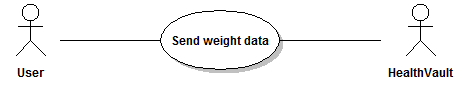
\includegraphics[scale=0.75]{../Figures/use-case-diagram-weight-service-send.png}
\caption{Use case diagram - HealthVault Integration Service send to HealthVault}
\label{figure:use-case-diagram-weight-service-send}
\end{figure}

\begin{table}[H]
\begin{center}
\begin{tabular}{ l | p{10cm} }
  \hline
  \textbf{Use Case Element} & \textbf{Description} \\ \hline\hline
  Requirements & \hyperref[table:reqwebservice]{FHIS1}\\ \hline
  Application & HealthVault Integration Service \\ \hline
  Name & Send weight to HealthVault \\ \hline
  Description & Send a weight measurement from the web service into HealthVault. \\ \hline
  Actor & User and HealthVault\\ \hline
  Precondition &
    \par 1. The user has logged in to HealthVault through the web service.
  \\ \hline
  Basic Flow & 
  	\par 1. The user enters a weight value into the weight field.
  	\par 2. User clicks on the send button.
  	\par 3. HealthVault receives the data.
  \\ \hline
\end{tabular}
\end{center}
\caption{Textual use case - Send weight to HealthVault}
\label{table:use-case-send-weight-to-healthvault}
\end{table}

In figure \ref{figure:use-case-diagram-weight-service-poll} an overview is given of the polling service.
Table \ref{table:use-case-start-polling-service} shows a textual use case for the polling functionality.

\begin{figure}[H]
\centering
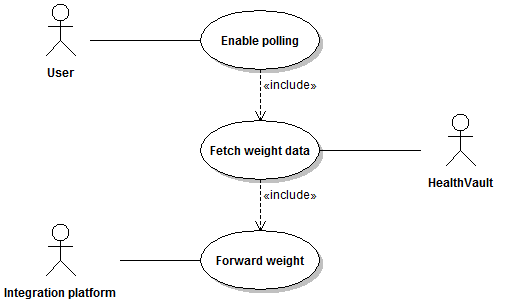
\includegraphics[scale=0.75]{../Figures/use-case-diagram-weight-service-poll.png}
\caption{Use case diagram - HealthVault Integration Service data polling}
\label{figure:use-case-diagram-weight-service-poll}
\end{figure}

\begin{table}[H]
\begin{center}
\begin{tabular}{ l | p{10cm} }
  \hline
  \textbf{Use Case Element} & \textbf{Description} \\ \hline\hline
  Requirements & \hyperref[table:reqwebservice]{FHIS2}, \hyperref[table:reqwebservice]{FHIS3} and \hyperref[table:reqip]{FIP2}\\ \hline
  Application & HealthVault Integration Service \\ \hline
  Name & Start polling service \\ \hline
  Description & Start the polling service and send data from HealthVault to the integration platform. \\ \hline
  Actor & User, HealthVault and Integration Platform \\ \hline
  Precondition &
    \par 1. The user has logged in to HealthVault through the web service.
    \par 2. The polling service is off.
  \\ \hline
  Basic Flow & 
  	\par 1. The user clicks on \textit{Enable} button to start the polling service.
  	\par 2. The web service polls data from HealthVault.
  \\ \hline
   Alternate Flows & 
  	\par 2A: No new weight measurement.
  	\par\hspace{15pt} 1. Go to 2 and poll again.
  	\par 2B: New weight measurement detected.
  	\par\hspace{15pt} 1. Send new weight data to integration platform.
  	\par\hspace{15pt} 2. Integration platform receives data.
  	\par\hspace{15pt} 3. Go to 2 and poll again.
  \\ \hline
\end{tabular}
\end{center}
\caption{Textual use case - Start polling service}
\label{table:use-case-start-polling-service}
\end{table}

%\section{Test plan}
%\label{section:testplan}

%Most of the testing was performed manually.
%Since the product consisted of two Android applications and a Spring
